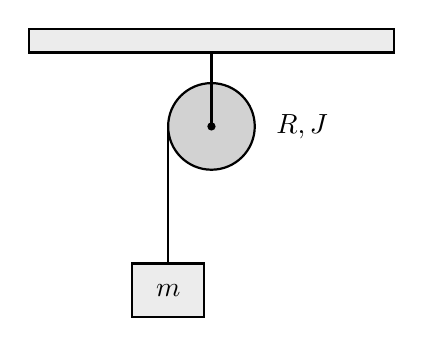
\begin{tikzpicture}
  \draw[fill=gray!15,thick] (-2.32,1.74) rectangle (2.32,2.04);
  \draw[fill=gray!35,thick] (0,0.80) circle[radius=0.55];
  \draw[thick] (0,1.74) -- (0,0.80) (-0.55,0.80) -- (-0.55,-0.94);
  \fill (0,0.80) circle[radius=1.5pt];
  \node[right] at (0.70,0.80) {$R, J$};
  \draw[fill=gray!15,thick] (-1.01,-0.94) rectangle (-0.09,-1.62);
  \node at (-0.55,-1.28) {$m$};
\end{tikzpicture}
